\begingroup
\titleformat{\chapter}[display]{\normalfont\Huge\bfseries\raggedright\setstretch{1}}{}{0pt}{}
\titlespacing*{\chapter}{0pt}{0pt}{12pt}
\titleformat{\section}{\normalfont\Large\bfseries\raggedright\setstretch{1}}{\thesection}{.7em}{}
\titleformat{\subsection}{\normalfont\large\bfseries\raggedright\setstretch{1}}{\thesubsection}{.7em}{}
\titlespacing*{\section}{0pt}{14pt}{6pt}
\titlespacing*{\subsection}{0pt}{10pt}{4pt}
\setlength{\parskip}{5pt}
\setlength{\parindent}{0pt}
\setlength{\emergencystretch}{2em}
\raggedbottom
\widowpenalty=10000\clubpenalty=10000
\providecommand{\CombinedFullAppendix}{\ifcsname r@explain:app_full\endcsname Appendix~\ref{explain:app_full}\else the full-weld explanatory appendix\fi}
\providecommand{\CombinedPartialAppendix}{\ifcsname r@explain:app_partial\endcsname Appendix~\ref{explain:app_partial}\else the partial-weld explanatory appendix\fi}

\chapter{Simulations of laser-ultrasonic imaging of full and partial welds using COMSOL and SAFT}
\chaptermark{Laser-ultrasonic imaging of full and partial welds}
\label{combinedex:chapter}

\section{Research question and approach}
\label{combinedex:intro}
Laser generation and optical reception offer a way to inspect a weld without a contacting ultrasonic probe. The relevant measurement is the surface motion produced by a laser-generated elastic wave after propagation and scattering. Laser synthetic arrays and laser-ultrasonic weld imaging provide experimental precedents for this approach~\cite{stratoudaki,levesque}. Here the question is narrower and testable: do physically plausible laser sources and normal-motion receivers contain enough acoustic information to localize an embedded LOF in either a completed or a partly filled weld?

The two weld states differ in more than the amount of material. In the full weld, all acquisition positions lie on a continuous outer surface. In the partial weld, the exposed weld surface lies inside an open groove. It brings some sources close to the flaw, but blocks some direct routes to the outer receivers. A propagation path that is useful in one state may therefore be weak, poorly timed or physically impossible in the other. The study examines source locations, receiving surfaces and imaging paths together.

The workflow has three distinct stages. First, a small thermoelastic COMSOL model calibrates an equivalent laser source without using the flaw. This is done to reduce computation time. Second, COMSOL models propagate that source in flawed and pristine specimens. Third, a separate C++ SAFT calculation focuses the exported recordings according to declared paths and selection rules. 

This chapter explains the shared model and construction, then compares the resulting acquisition strategies. The complete simulation descriptions, path comparisons, filter comparisons, settings and numerical controls are provided in appendix A a fully worked out SAFT workflow example is in XX, and can be useful to understand the analysis. 

\section{Geometries, laser acquisition and COMSOL model}
\label{combinedex:model}
\subsection{Partial and full weld geometry}
Figure~\ref{combinedex:geometry} compares the two geometries, which are replicas of the physically acquired samples. Each is 150 mm wide and 25.4 mm thick. Depth $z$ is measured downwards from the original outer surface; $x=0$ is the weld centre. The J preparation has a 7.1068 mm opening, a 4.7 mm entrance section, shallow $3^\circ$ flanks and a rounded root reaching approximately 24.061 mm depth. The internal weld outline is bonded to the surrounding material except at the prescribed separation. The full weld is filled to $z=0$. The 9 mm partial fill leaves an exposed weld surface at $z=16.4$ mm, between approximately $x=\pm2.940$ mm.

The LOF lies on the right flank. Its upper and lower tips are at $(x,z)=(2.831875,18.467475)$ and $(2.700855,20.967475)$ mm. Its vertical extent is 2.5 mm and its length along the flank is 2.5034 mm. The lower tip remains 4.4325 mm above the backwall. The flaw is represented by traction-free faces, meaning no contact closure or friction is included. This same segment is used in both weld states, which isolates the effect of the acquisition geometry and fill state rather than introducing a different defect.

\begin{figure}[!htbp]\centering
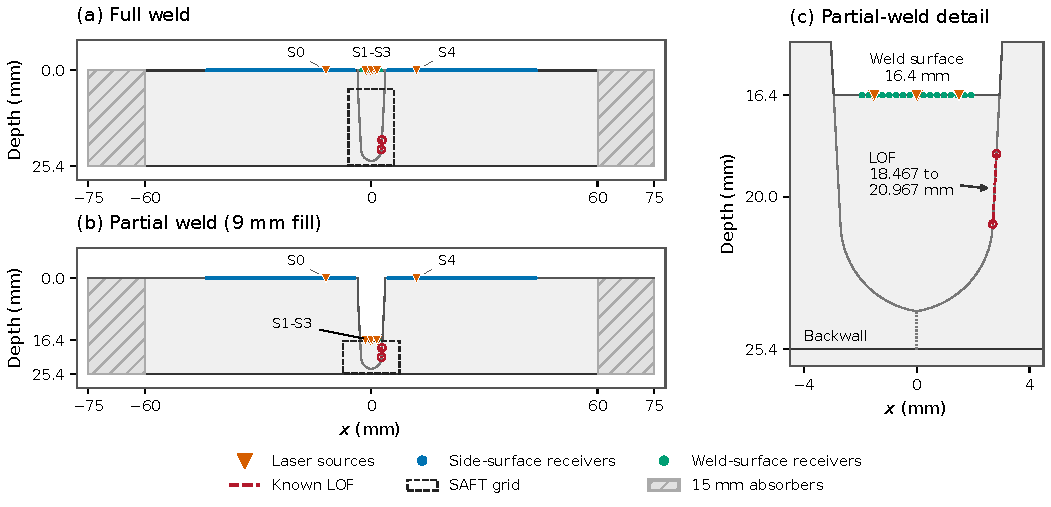
\includegraphics[width=\linewidth]{figures/combined_explanatory/geometry.pdf}
\caption{Specimen geometry and acquisition. Orange triangles identify the two shoulder sources S0/S4 and three weld-surface sources S1--S3. Blue and green points denote side-surface and weld-surface receivers. The specimens include 15 mm absorbing strips at each lateral end. Separate dashed boxes show the actual full- and partial-weld reconstruction fields. The enlarged partial-weld detail shows the exposed floor, continuous J root and prescribed LOF. The grey internal outline is bonded except along the red flaw segment; it is not an open groove boundary below the fill.}
\label{combinedex:geometry}
\end{figure}

The five source coordinates are $x=-12,-1.5,0,1.5,12$ mm. S0 and S4 are shoulder sources at the original outer surface. S1--S3 lie on the exposed weld surface: $z=0$ in the full weld and $z=16.4$ mm in the partial weld. Both specimens have 157 receivers on each side surface at 0.25 mm pitch, extending to approximately $x=\pm43.5534$ mm. There are also 23 full-weld or 17 partial-weld receivers on the central weld surface, giving 337 and 331 receivers respectively. Every receiver measures the  vertical velocity $v_y$.

Five flawed and five pristine source simulations are made for each weld state: twenty production solves in total. This means each source is separately modelled and they can't affect each other. Every recording contains 5001 samples over 50 $\mu$s at 10 ns output spacing. A pristine simulation has the same geometry and source but no LOF. It provides control and allows for signed waveform subtraction. It is also not an input to the LOF-only defect imaging algorithm. This is important because experimentally a pristine sample analysis will be very hard to require. Therefore abusing this information in the simulations is not useful. 

\subsection{Elastic propagation}
Simulations are done in COMSOL Multiphysics 6.4, with the Elastic Waves, Time Explicit interface. Steel is homogeneous, isotropic and linearly elastic, under two-dimensional plane strain. The model uses $E=212.443$ GPa, $\nu=0.288978$ and $\rho=7859.975$ kg\,m$^{-3}$, giving longitudinal and in-plane shear speeds of $c_L=5943.60$ and $c_S=3237.97$ m\,s$^{-1}$. The corresponding Rayleigh speed used for arrival screening is $c_R=2997.33$ m\,s$^{-1}$. Longitudinal motion is primarily parallel to propagation; shear motion is transverse. Both can contribute to measured normal surface velocity after interaction with a free surface.

The elastic field satisfies
\begin{equation}
 \rho\,\ddot{\mathbf u}=\nabla\!\cdot\boldsymbol\sigma,
 \qquad \boldsymbol\sigma=\lambda\,\mathrm{tr}(\boldsymbol\varepsilon)\mathbf I
                 +2\mu\boldsymbol\varepsilon,
 \qquad \boldsymbol\varepsilon=\tfrac12(\nabla\mathbf u+\nabla\mathbf u^{\top}).
\end{equation}
Here $\mathbf u$ is displacement and $\lambda,\mu$ are the Lam\'e constants. Exposed surfaces and the LOF are traction-free except where the equivalent source acts. Bonded internal boundaries transmit displacement and traction. Weld and surrounding steel have identical properties. Absorbing strips at the lateral ends reduce artificial returns from the truncated specimen, that would not be present in a round pipe.

The numerical discretization uses quartic velocity and strain fields, a discontinuous Galerkin formulation and explicit fourth-order Runge--Kutta integration. Maximum element sizes are approximately 0.32380 mm in the weld and 0.48570 mm in the surrounding material, chosen using a 5 MHz simulation resolve frequency. Higher frequency could contain more information, however experimentally they attenuate faster \cite{wan-2017}. Simulation runtime is also an important consideration, higher frequencies require smaller meshes and can cause smaller stable time steps \cite{comsol-elastic-mesh}. For our models runtime scales as \begin{equation}
    T(f) \approx T(5\,\mathrm{MHz})
    \left(\frac{f}{5\,\mathrm{MHz}}\right)^3.
    \label{eq:runtime_frequency_scaling}
\end{equation}
This means increasing the frequency to 10 MHz leads to approximately eight times the runtime.

\subsection{Laser-equivalent source}
\label{combinedex:calibration}
The laser source is represented by an equivalent tangential traction that approximates thermoelastic expansion from an absorbed laser line, following the surface-force-dipole approach described by Tu et al.~\cite{tu}. Its amplitude is calibrated against a thermoelastic calculation. The calibration uses a flat domain measuring 8~mm in width and 4~mm in depth. COMSOL Heat Transfer in Solids connects the temperature field to Solid Mechanics through thermal expansion. A second mechanical field on the same mesh receives the equivalent traction.

For the Gaussian spatial profile, define $\xi=(x-x_s)/w$, where $x_s$ is the source centre and $w=0.5$~mm is the prescribed $1/e^2$ half-width. The temporal profile uses the 6.5~ns pulse duration reported for the laser system of Yu et al.~\cite{yu-2021}. Here, this duration is interpreted as the Gaussian full width at half maximum. The absorbed heat flux is
\begin{equation}
 q(x,t)=\frac{F_0}{\sqrt{2\pi}\sigma_t}
 \exp(-2\xi^2)
 \exp\!\left[-\frac{(t-t_0)^2}{2\sigma_t^2}\right],
 \qquad
 \sigma_t=\frac{6.5\ \mathrm{ns}}{2\sqrt{2\ln2}}.
\end{equation}
The pulse centre is prescribed at $t_0=30$~ns so that the short Gaussian pulse lies inside the simulated time window.  The parameter $F_0$ denotes the peak absorbed fluence, set to 100~J\,m$^{-2}$. The source half-width and absorbed fluence are choices.

The equivalent surface load is a tangential dipole,
\begin{equation}
 t_x(x,t)=4A\xi e^{-2\xi^2}H(t),\qquad t_y=0,
 \qquad
 H(t)=\tfrac12\left[
 1+\operatorname{erf}\!\left(
 \frac{t-t_0}{\sqrt2\sigma_t}
 \right)\right],
\end{equation}
with
\begin{equation}
 A=\gamma\frac{E\alpha F_0}{(1-\nu)\rho c_p w}.
\end{equation}
The opposing tangential lobes represent the lateral expansion of a thin heated region. The function $H(t)$ is the time integral of the normalized Gaussian power pulse, consistent with the equivalent-source formulation~\cite{tu}. Retaining the finite source width accounts for its influence on the angular and frequency response.

The thermal calculation starts from $T_0=293.15$~K. Thermal conductivity is 52~W\,m$^{-1}$\,K$^{-1}$, specific heat capacity is $c_p=480$~J\,kg$^{-1}$\,K$^{-1}$, and the linear thermal expansion coefficient is $\alpha=11\times10^{-6}$~K$^{-1}$. These three material properties are taken from the X65 data reported by Dölz et al.~\cite{dolz-2024}. The elastic modulus
$E$, Poisson ratio $\nu$ and density $\rho$ are retained from the weld model.

Only the scalar gain $\gamma$ is fitted. Signed horizontal and vertical velocity histories at five points on a 2~mm radius arc, from $15^\circ$ to $75^\circ$, are compared over 0.12--0.82~$\mu$s. Both fields receive the same forward--backward fourth-order 5~MHz Butterworth filter for this calibration comparison. If $\mathbf d$ is the vector of filtered unit-gain dipole histories and $\mathbf v$ the corresponding thermoelastic histories, the least-squares
result is
\begin{equation}
 \gamma=
 \frac{\mathbf d^{\top}\mathbf v}
      {\mathbf d^{\top}\mathbf d}
 =1.084434.
\end{equation}
Figure~\ref{combinedex:source} compares the dipole source with the thermoelastic simulation. After fitting a single amplitude factor, the relative difference between their velocity waveforms is 0.931\%. At two additional receiver positions that were not used in the fit, the differences are 1.09\% for the axial receiver and 1.27\% for the surface receiver. This agreement supports using the simpler dipole source within the tested frequency band.

At the prescribed absorbed fluence of 100~J\,m$^{-2}$, the calibrated amplitude coefficient is $A=188.939$~kPa.
This gives a maximum force per unit surface area of 229.195~kPa.

\begin{figure}[!htbp]
\centering
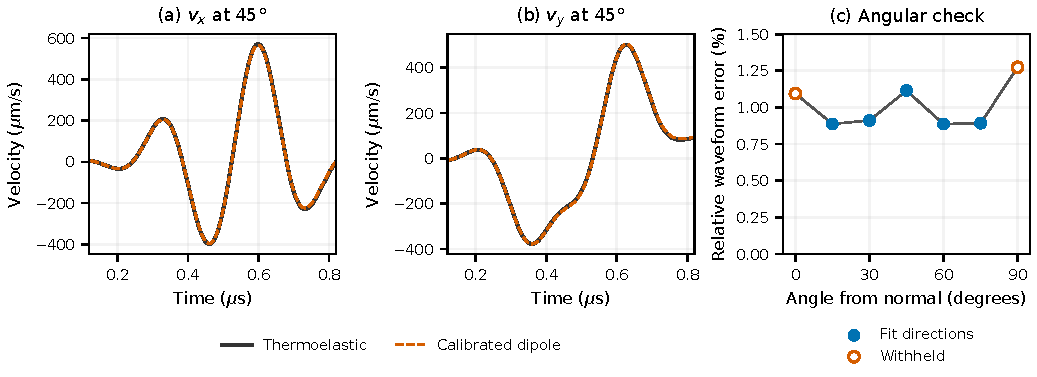
\includegraphics[width=.96\linewidth]
{figures/combined_explanatory/source_calibration.pdf}
\caption{Independent source calibration. The equivalent
traction is assessed through comparisons of signed outgoing
velocity histories and angular response with the
thermoelastic calculation. A single gain scales the dipole,
without using a reconstructed flaw image. Agreement supports using this dipole as a substitute laser generation}
\label{combinedex:source}
\end{figure}

The thermal mesh resolves the thin heated layer with nine layers totalling 25.55~$\mu$m. The calibration uses implicit generalized-$\alpha$ integration, with maximum steps of 0.5~ns initially and 2~ns after. Its absorbed energy agrees with the Gaussian input within 0.000639\%, and the temperature rise at 100~J\,m$^{-2}$ is 78.34~K. These checks and the outgoing waveform comparison support transferring the equivalent source to the larger weld model. Calibration of a physical laser instrument remains a separate requirement and could not be done since a generation laser was not obtained.

\section{SAFT imaging}
\label{combinedex:method}
SAFT asks whether different receiver histories contain motion at the times expected if ultrasound scattered at a trial pixel $\mathbf p$. For each source $s$, receiver $r$ and chosen path $P$, it predicts
\begin{equation}
 T_{sr,P}(\mathbf p)=t_0+\sum_{j\in P}\frac{\ell_j(\mathbf p)}{c_{m_j}},
\label{combinedex:delay}
\end{equation}
where each leg has length $\ell_j$ and mode $m_j\in\{L,S\}$. The path notation places a vertical bar at the trial scattering point. Thus $S\mid S$ is direct shear illumination and direct shear reception; $S\mid SS$ adds one backwall reflection on the receiving route; $SS\mid S$ adds it on the incident route. $L\mid L$ is the direct longitudinal view.

Every segment must remain in steel and every reflection must lie on an actual boundary. In the partial weld, a ray cannot cross the open groove. Valid routes use the original surface, the exposed fill floor or the backwall. The source and receiver sets are evaluated at every image pixel in the SAFT grid.

\begin{figure}[!htbp]\centering
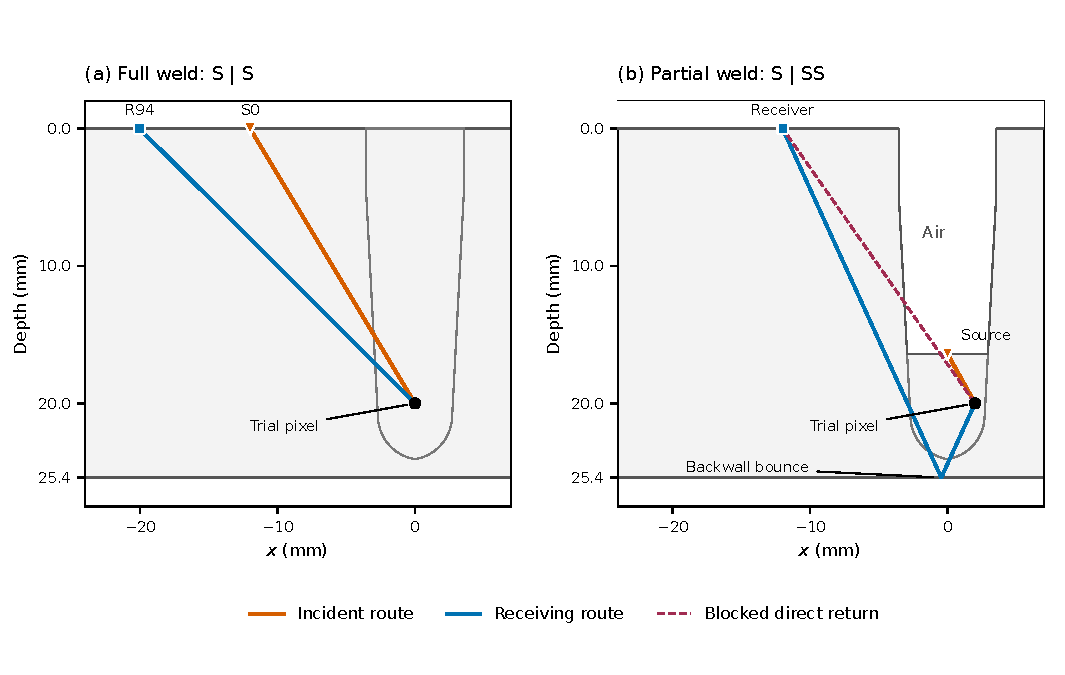
\includegraphics[width=.98\linewidth]{figures/combined_explanatory/path_examples.pdf}
\caption{Illustrative paths. (a) A full-weld $S\mid S$ route from a shoulder source to a trial pixel and side receiver. (b) In the partial weld, direct illumination from the weld surface and a backwall-reflected return can remain inside steel even when a direct return crosses the open groove.}
\label{combinedex:paths}
\end{figure}

For example, a full-weld source at $(-12,0)$ mm, receiver at $(-20.0534,0)$ mm and pixel at $(0,20)$ mm give a direct-S delay of about 15.98 $\mu$s; the same lengths give about 8.72 $\mu$s for direct L. In the partial-weld example, a source at $(0,16.4)$ mm illuminates $(2,20)$ mm and returns through a backwall bounce to an illustrative receiver at $(-12,0)$ mm. The incident length is 4.118 mm and the reflected receiving length is 33.833 mm, giving $T=11.751$ $\mu$s. The direct return would cross the fill depth at $x=-0.52$ mm, inside the open groove, and is invalid. The reflected return crosses that depth at about $x=-7.91$ mm, in steel. 

\subsection{Generation and detection angles}
A laser dipole does not launch all modes equally in all directions. A normal-motion receiver also does not observe every incoming mode equally. Free-surface reflection and conversion contribute to its response, so normal sensitivity cannot be estimated from the incident displacement component alone. Therefore, we use the angular magnitudes in Figure~\ref{combinedex:coupling} to admit plausible paths.

\begin{figure}[!htbp]\centering
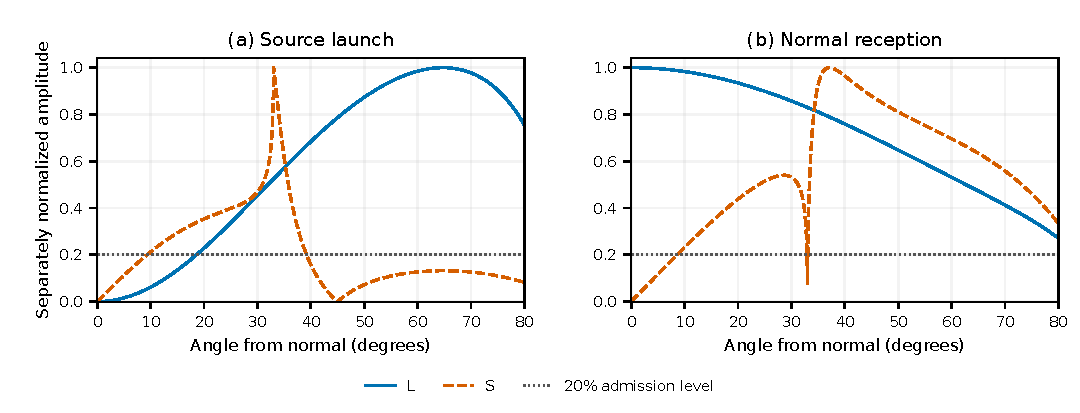
\includegraphics[width=.92\linewidth]{figures/combined_explanatory/coupling.pdf}
\caption{Angular launch and normal-reception magnitudes used for channel admission. L and S are normalized separately, so the curves do not compare absolute longitudinal and shear energy. The 20\% level is a selection threshold: a channel must satisfy both its source and receiver tests. Admitted receivers are subsequently averaged equally. These curves explain why a large spatial aperture can still contain unsuitable mode/path combinations.}
\label{combinedex:coupling}
\end{figure}

For a path to qualify, both normalized launch and receive magnitudes must reach 20\%, and receive angle must not exceed $80^\circ$ from the normal. A reflected route must also pass a 5\% wall-response-product gate. These are modelling choices, not amplitude weights or phase corrections. A 1.5 mm source--receiver separation exclusion keeps receivers outside the approximately 1.425 mm source-footprint half-width. 

\subsection{Frequency filtering and pulse-aware screening}
\label{combinedex:time}
The recorded field includes direct bulk waves, surface motion, reflected packets and flaw scattering. A strong direct packet can be sampled at a delay assigned to a deep trial pixel and create an apparent indication. Its coherence across receivers means that ordinary averaging, or even coherence weighting, may preserve it. This contamination is therefore a mismatch between the packet's actual route and the route assumed in focusing. 

The basic SAFT uses an analytic FIR filter over $0.5$--$5\,\mathrm{MHz}$. It reduces slowly varying motion and
high-frequency content while retaining amplitude and phase for delay-and-sum processing. The upper cutoff follows the frequency range used for mesh design and source calibration. The Kaiser design targets $55\,\mathrm{dB}$ stopband attenuation with a $0.5\,\mathrm{MHz}$ transition width, giving 657 taps and $\beta=5.10226$~\cite{kaiser-1974,scipy-kaiserord}. At $10\,\mathrm{ns}$ sample spacing, filtering requires $3.28\,\mu\mathrm{s}$ of data on either side of each sample. Therefore, usable time ranges are $3.28$--$46.71\,\mu\mathrm{s}$. This filter is again a design choice and not established as the optimal, however different filters were also investigated.

Direct L, S and Rayleigh arrivals are then screened per source--receiver pair. A geometry-valid prediction locates an envelope peak within $\pm0.25$ $\mu$s. The packet window extends until the envelope is below $-30$ dB relative to that peak for at least 0.15 $\mu$s, with a further 0.1 $\mu$s margin. An imaging sample falling within the excluded window is not admitted. This avoids a single fixed mute duration for packets with different widths. Rayleigh screening requires a common unobstructed flat surface; it does not assume a surface wave crosses the empty groove.

These rules affect the geometries differently. All 1685 full-weld source--receiver pairs have direct bulk paths. Only 365 of 1655 partial-weld pairs have direct paths: shoulder-to-side pairs on their own side and weld-surface pairs on the floor. 

The screening windows for an LOF-only image are obtained from its own recording. A pristine image uses its own windows; the waveform-difference control uses the LOF-derived windows. The procedure therefore requires no reference recording to suppress the direct field. It can still reject real flaw information when arrivals overlap, especially for a source close to the partial-weld flaw. 

\subsection{Coherence and source coverage}
Let $a_{sr}(\mathbf p)$ be the complex filtered history interpolated at Equation~\ref{combinedex:delay}, after the channel and timing tests. For $N_s$ admitted receivers, the equal mean and receiver coherence factor are
\begin{equation}
 M_s(\mathbf p)=\frac{1}{N_s}\sum_r a_{sr}(\mathbf p),\qquad
 \mathrm{CF}_s(\mathbf p)=\frac{|\sum_r a_{sr}(\mathbf p)|^2}
 {N_s\sum_r|a_{sr}(\mathbf p)|^2}.
\label{combinedex:cf}
\end{equation}
The coherence factor is zero for zero signal energy and otherwise lies between zero and one. Aligned phases reinforce in the numerator; inconsistent phases reduce it. It encourages phase consistency under the selected delay law, but a coherent structural echo can also pass that test. 

Each source must retain at least eight receivers and at least 25\% of its aperture eligible before the time-support and pulse tests, again these are choices. Furthermore, the image requires at least two qualifying sources at a pixel. If $\mathcal S(\mathbf p)$ is that set, source results combine as
\begin{equation}
 I(\mathbf p)=\left[\frac{1}{|\mathcal S|}\sum_{s\in\mathcal S}
                 |\mathrm{CF}_s M_s|^2\right]^{1/2}.
\label{combinedex:source_rms}
\end{equation}
This root-mean-square combination avoids cancellation between separately illuminated source views. The output retains velocity units but is a processed focusing score, not acoustic intensity or flaw size. A pixel failing the required source count is unsupported and is coloured grey.

Allowing one qualifying source changes which pixels can be displayed. It does not mean acquiring only one laser shot for the whole image: all selected source shots remain available wherever they qualify, and Equation~\ref{combinedex:source_rms} still uses them. This distinction is essential to the partial-weld coverage comparison below.

\subsection{SAFT images and controls}
\label{combinedex:metrics}
The full-weld SAFT grid spans $x=\pm6$ mm and depths 5--25.25 mm, the partial-weld grid spans $x=\pm7.5$ mm and 16.65--25.25 mm depth. Images use 0.1 mm pixels. At 5 MHz the shear wavelength is approximately 0.648 mm, so the pixel grid samples the image finely but does not establish 0.1 mm physical resolution. Finer 0.05 mm grids and wider $x=\pm45$ mm fields check peak stability and competing indications.

The images show $20\log_{10}[I(\mathbf p)/I_0]$ over a declared display range: 45 dB for the principal path and source-threshold panels, and 40 dB for the partial-weld acquisition comparison. A shared reference is used within each comparison. Black denotes low displayed amplitude, grey denotes unsupported material, and white denotes air. External LOF guides identify the flaw location. 

Define a near-flaw region $\mathcal N$ within 0.5 mm of the flaw and a background region $\mathcal B$ more than 1 mm from it. Over supported pixels,
\begin{equation}
 C_{\max}=20\log_{10}\frac{\max_{\mathcal N}I}{\max_{\mathcal B}I},\qquad
 C_{99}=20\log_{10}\frac{\max_{\mathcal N}I}{Q_{99,\mathcal B}(I)}.
\end{equation}
Positive $C_{\max}$ means the strongest near-flaw response exceeds every assessed background pixel. Changing an aperture changes both the signal and the assessed region; comparisons therefore report support and, where needed, restrict both images to a common mask.

The LOF-only image is the main result. Pristine images test whether the reference produces a similar indication. Difference controls subtract signed LOF and pristine waveforms before filtering and focusing. Since interference and coherence change, a difference image can have a larger peak than the LOF-only image. These controls support attribution to the flaw.

\section{Full weld results}
\label{combinedex:full}

\begin{figure}[!htbp]\centering
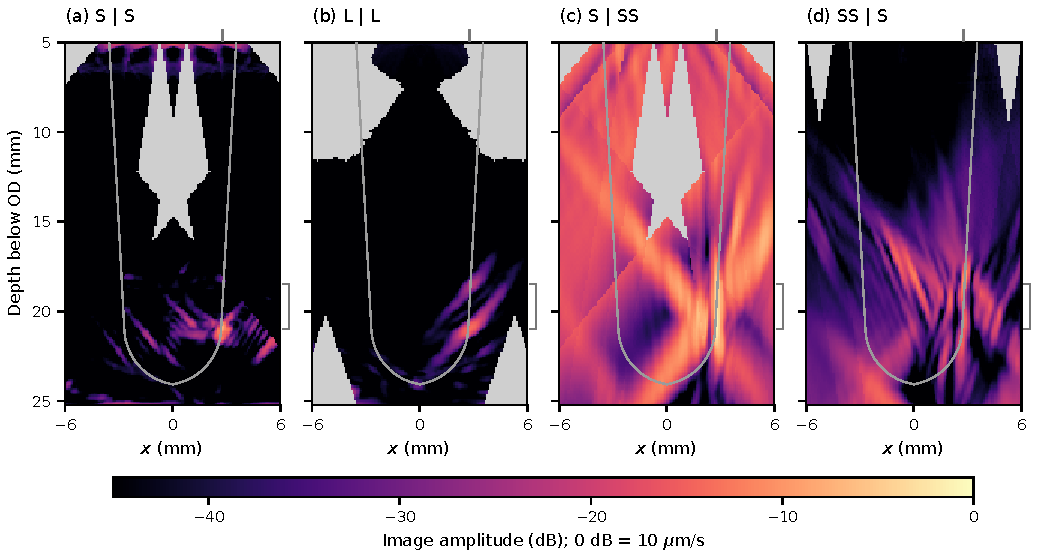
\includegraphics[width=\linewidth]{figures/combined_explanatory/full_common_paths.pdf}
\caption{Full-weld LOF-only images for four paths using the same 657-tap 0.5--5 MHz filter, screening, coupling and support rules. All panels use 0.1 mm pixels, 0 dB = 10 $\mu$m/s and a 45 dB range. Direct paths emphasize the lower-tip vicinity; reflected paths give more extended indications. Grey pixels fail the declared coverage rules. Different paths admit different rays even when their selection rules are identical.}
\label{combinedex:full_paths}
\end{figure}

Figure~\ref{combinedex:full_paths} shows SAFT images for different paths with the same settings. All four paths produce a global maximum within 0.37 mm of the prescribed LOF and support the entire evaluated near-flaw region. Their $C_{\max}$ values are 8.85 dB for $L\mid L$, 6.47 dB for $S\mid S$, 4.65 dB for $S\mid SS$ and 4.37 dB for $SS\mid S$. The images provide complementary views of the defect. Tweaking of the background controls and combining these images could allow for defect sizing, but this is not done in this analysis.

The direct images mainly emphasize the tips. A nearly vertical defect does not necessarily return a strong  reflection to the generating surface, as tip scattering and oblique illumination matter. More extended reflected-path indications are consistent with different angular access, as in backwall-assisted imaging strategies~\cite{nicolson23}. 

\subsection{Direct-shear interpretation}
For direct S, changing the 657-tap common bandpass to a 257-tap bandpass with the same nominal edges increases $C_{\max}$ from 6.47 to 10.26 dB. The 257-tap 0--5 MHz low-pass gives 12.79 dB. All use the same 3.28 $\mu$s admission guard, so this gain is not obtained by simply allowing earlier samples. Filter duration and retained frequency content change the waveforms being summed and their overlap with unwanted arrivals. The choice is path-specific: direct L gives only 3.24 dB with the short low-pass, compared with 8.85 dB under the FIR bandpass.

\begin{figure}[!htbp]\centering
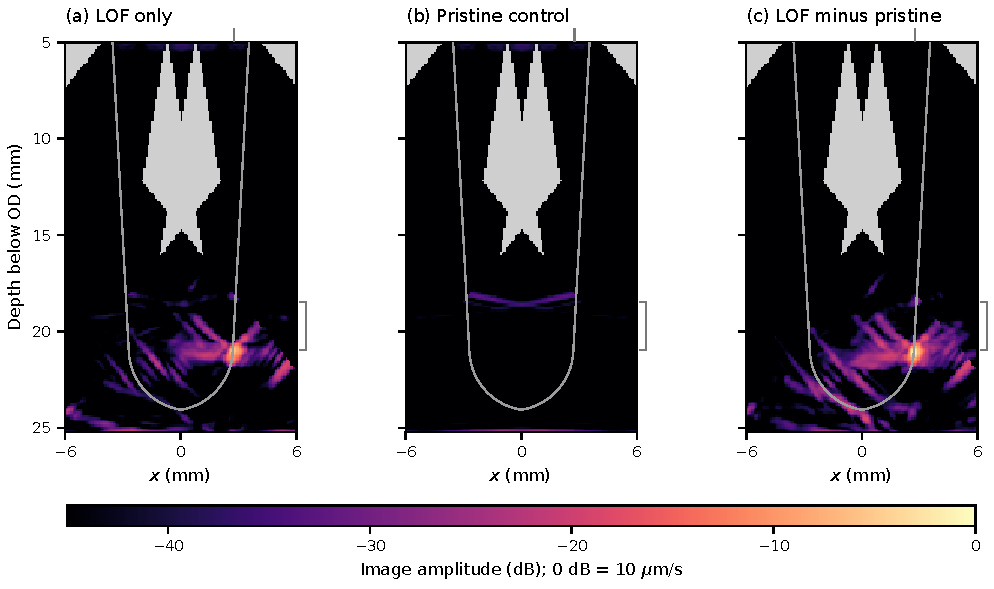
\includegraphics[width=\linewidth]{figures/combined_explanatory/primary_full.pdf}
\caption{Selected full-weld $S\mid S$ image, pristine control and signed-waveform-difference control. The short 0--5 MHz analytic FIR is used with the retained 3.28 $\mu$s guard. All panels have 0 dB = 10 $\mu$m/s and a 45 dB range. The LOF-only image localizes near the lower tip without reference subtraction; the pristine panel has no physical flaw. External marks show LOF location.}
\label{combinedex:full_selected}
\end{figure}

Figure~\ref{combinedex:full_selected} compares the direct S SAFT images. The LOF-only peak is 5.184 $\mu$m/s at $(2.7,21.0)$ mm, 0.0325 mm from the finite LOF segment. $C_{\max}=12.79$ dB, $C_{99}=21.28$ dB and near-flaw support is 100\%.  The pristine maximum is 0.485 $\mu$m/s and not near the defect. The difference maximum is 8.791 $\mu$m/s near the lower tip. The three panels together support a defect localisation in the LOF only image.

At a smaller pixel space of 0.05 mm spacing, contrast is 12.63 dB. Over a wider SAFT grid of  $x=\pm45$ mm field with 0.25 mm spacing, it is 10.62 dB and the global maximum remains near the flaw. The selected direct-S interpretation is therefore not restricted to one SAFT grid or pixel interval. This does not hold for every path. The  $SS\mid S$ path has a stronger lateral artefact in its wider field, giving $-17.80$ dB contrast. Additional paths should be retained for useful geometric information, rather than combined them without care.

\subsection{Source and receiver sensitivity}
Table~\ref{combinedex:full_groups} summarizes tests that remove whole source or receiver groups with the selected processing rules. These tests ask which surfaces carry useful information, rather than finding individual combinations that maximize the known-flaw score.

\par\medskip\noindent\begin{minipage}{\linewidth}\centering\small
\captionof{table}{Full-weld acquisition reductions for selected direct S. Side receivers comprise the two 157-position outer groups. The contrast uses each configuration's supported field, so support must be read alongside it.}
\begin{tabularx}{\linewidth}{@{}XXrr@{}}\toprule
Sources & Receivers & $C_{\max}$ (dB) & Near support (\%)\\\midrule
All five & All 337 & 12.79 & 100.0\\
Two shoulders & All 337 & 10.57 & 92.4\\
All five & Side surfaces & 11.83 & 100.0\\
Two shoulders & Side surfaces & 9.61 & 92.4\\
Three weld-surface & All 337 & $-20.66$ & 9.8\\
\bottomrule\end{tabularx}
\label{combinedex:full_groups}
\end{minipage}\par\medskip

Shoulder generation and side-surface reception retain a useful indication at 9.61 dB with 92.4\% near-flaw support. Generation or reception directly over the full weld is therefore not essential for this defect. Conversely, the three weld-surface sources alone provide poor direct-S coverage and negative contrast. Suitable oblique launch and receive angles, rather than source proximity alone, determine the useful aperture.

\section{Partial weld results}
\label{combinedex:partial}
Direct shear illumination followed by a backwall-reflected shear return, so  $S\mid SS$, provides a useful view of the partial-weld defect. As shown in Figure~\ref{combinedex:paths}, sources on the weld surface can illuminate the nearby LOF, while the reflected return reaches outer receivers without crossing the empty groove. The results first establish the effect of source and receiver selection using the original equal-averaging method. They then show how revised processing improves contrast while retaining a good near-flaw support.

\subsection{Path and filter comparison}
Our analysis compared eighteen direct and reflected paths. With all five sources and all 331 receivers and the common 0.5--5 MHz filter, $S\mid SS$ image gives $C_{\max}=4.36$ dB and 95.8\% near-flaw support. Its peak is 16.568 $\mu$m/s at $(2.8,19.95)$ mm, 0.046 mm from the LOF. The pristine maximum lies elsewhere, while the signed-waveform-difference image also has a strong response near the defect. Changing only the filter gives similar results in the LOF-only images: 4.20 dB for 1--5 MHz, 4.29 dB for a shorter bandpass and 4.34 dB for a shorter low-pass. Shoulder sources alone provide no supported near-flaw image under the rules. With weld-surface sources and both receiving sides, $S\mid SS$ is the only one of the eighteen paths with positive contrast and a maximum near the flaw. 

\subsection{Source and receiver sensitivity}
\begin{figure}[!htbp]\centering
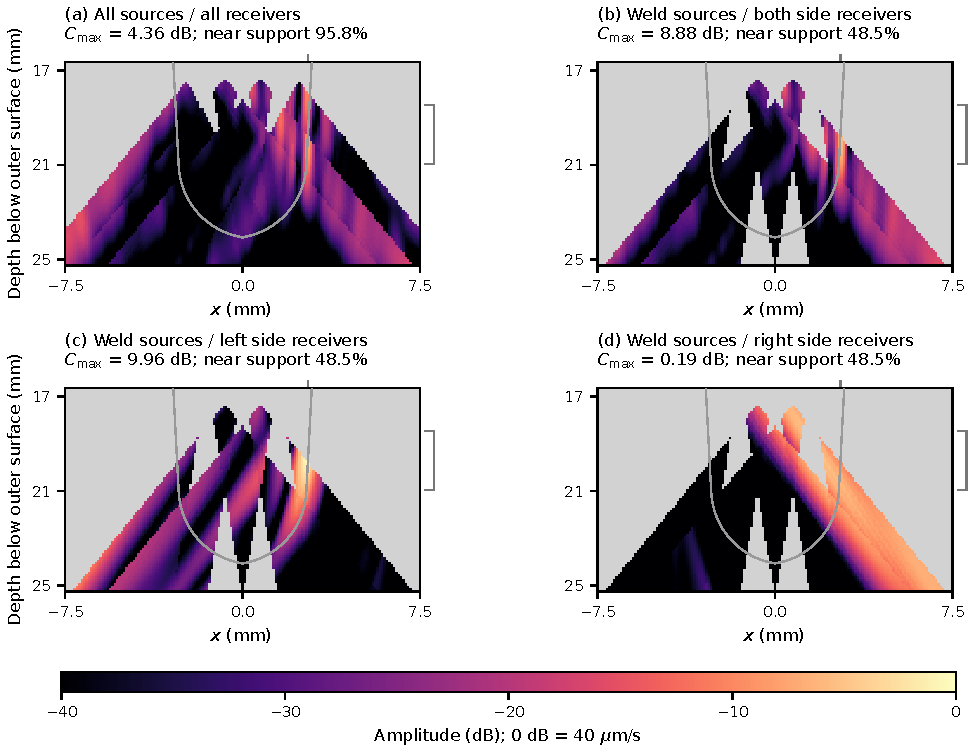
\includegraphics[width=\linewidth]{figures/combined_explanatory/partial_joint.pdf}
\caption{$S\mid SS$ acquisition comparison with equal averaging and a two-source minimum. All panels use 0 dB = 40 $\mu$m/s and a 40 dB range. Restricting generation to the three weld-surface sources reduces the supported region, shown in grey.}
\label{combinedex:partial_groups_fig}
\end{figure}

With the three weld-surface sources, left-side reception gives 9.96 dB contrast, both sides 8.88 dB and the right side 0.19 dB. All three support only 48.5\% of the near-flaw region (Figure~\ref{combinedex:partial_groups_fig} and Table~\ref{combinedex:partial_groups}). The right-side maximum is 0.664 mm from the flaw, outside the defined near region, so its slightly positive contrast is not sufficient evidence of useful localization.

\begin{table}[!htbp]\centering\small
\caption{Original partial-weld $S\mid SS$ results with equal receiver averaging, the common filter and 0.1 mm pixels. ``Weld'' means the three exposed weld-surface sources. Near support measures the assessed fraction of the region within 0.5 mm of the flaw, not the fraction of flaw length detected.}
\label{combinedex:partial_groups}
\begin{tabularx}{\linewidth}{@{}XXrrr@{}}\toprule
Sources & Receivers & Minimum & $C_{\max}$ & Near support\\
 & & sources & (dB) & (\%)\\\midrule
All five & All 331 & 2 & 4.36 & 95.8\\
All five & All 331 & 1 & 2.15 & 100.0\\
Weld & Both sides & 2 & 8.88 & 48.5\\
Weld & Both sides & 1 & 3.06 & 95.8\\
Weld & Left side & 2 & 9.96 & 48.5\\
Weld & Left side & 1 & 3.72 & 95.8\\
Weld & Right side & 2 & 0.19 & 48.5\\
\bottomrule\end{tabularx}
\end{table}

Some of the apparent benefit of left-only reception comes from leaving difficult pixels unassessed. On the same supported pixels, the all-source image gives 7.02 dB, making the left-side advantage 2.94 dB rather than the 5.60 dB difference between the unrestricted scores. Left-side contrast remains 10.26 dB at 0.05 mm spacing and 9.11 dB in the wider 0.25 mm field; both-side reception gives 9.20 dB in that wider field. Left reception is therefore useful for this acquisition, but is not generally superior to the other side.

Lowering the required number of qualifying sources from two to one increases left-side near support from 48.5\% to 95.8\%, but lowers contrast from 9.96 to 3.72 dB. The acquisition and all other processing settings remain fixed. Previously supported pixels are unchanged, and all new supported pixel have exactly one qualifying source. All three weld-source shots are still used wherever they qualify, so it's not that only one source is used, all of them are used but only one contribution is required.

\begin{figure}[!htbp]\centering
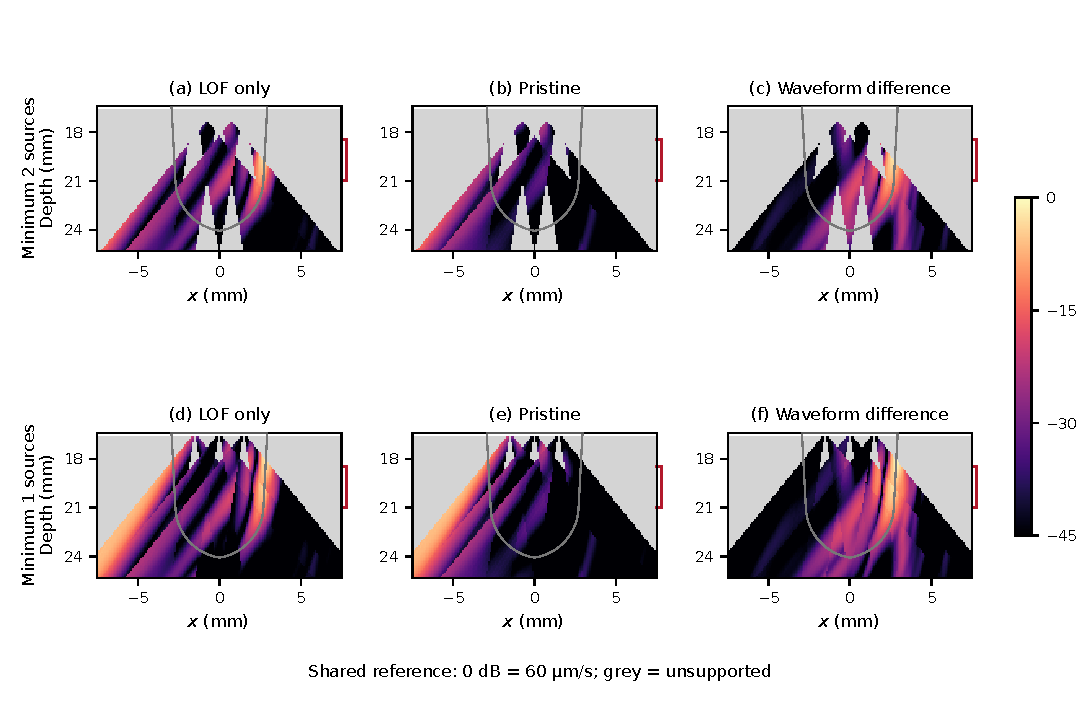
\includegraphics[width=\linewidth]{figures/combined_explanatory/partial_source_threshold.pdf}
\caption{Two-source and one-source requirements for the original $S\mid SS$ image, using three weld-surface sources and 157 left receivers. Columns show defect, pristine and signed-waveform-difference images. All panels use 0 dB = 60 $\mu$m/s and a 45 dB range. The one-source rule adds coverage and background without changing previously supported pixels.}
\label{combinedex:threshold}
\end{figure}

The one-source image reveals a stronger response near the upper tip, peaking at 46.152 $\mu$m/s at $(2.9,18.15)$ mm. It also admits a lateral background peak of 30.066 $\mu$m/s at $(-7.0,23.45)$ mm. The pristine maximum lies away from the flaw, with $-37.53$ dB contrast, while the difference image gives 10.02 dB. These controls support a flaw-related contribution, but the brighter near-flaw response does not make the image cleaner.

The left-side one-source contrast remains 3.73 dB at 0.05 mm spacing and 3.22 dB in the wider field, where near support is 94.3\%. Both-side reception gives 4.87 dB in that wider field. With all five sources and all receivers, allowing one source fills the near region but lowers contrast from 4.36 to 2.15 dB. Relaxing the source rule therefore trades a cleaner, smaller image for broader coverage. Near support is not the fraction of flaw length detected.

\subsection{Weighted receiver averaging}
Figure \ref{combinedex:partial_reassessment} shows an improved $S\mid SS$ image that uses all five sources and all receivers. Instead of averaging equally, it weights and phase-corrects the receiver samples using the predicted wall and normal detection values. The filter remains 657 taps long, but its band changes to 1--5 MHz and the angular threshold decreases from 20\% to 15\%. The two-source minimum, receiver-retention rules, coherence exponent of one, RMS source combination and direct-arrival screening are still the same as before.

Using these settings, contrast reaches 9.09 dB with 96.9\% near-flaw support on a 0.025 mm grid. A further improvement comes from a narrow mute around the predicted source--backwall--receiver $SS$ path, which does not pass through the trial pixel. Samples within $\pm0.225$ $\mu$s of this arrival are removed, with a smooth transition to full weight at $\pm0.30$ $\mu$s. Only this additional fixed mute is enabled.

\begin{figure}[!htbp]\centering
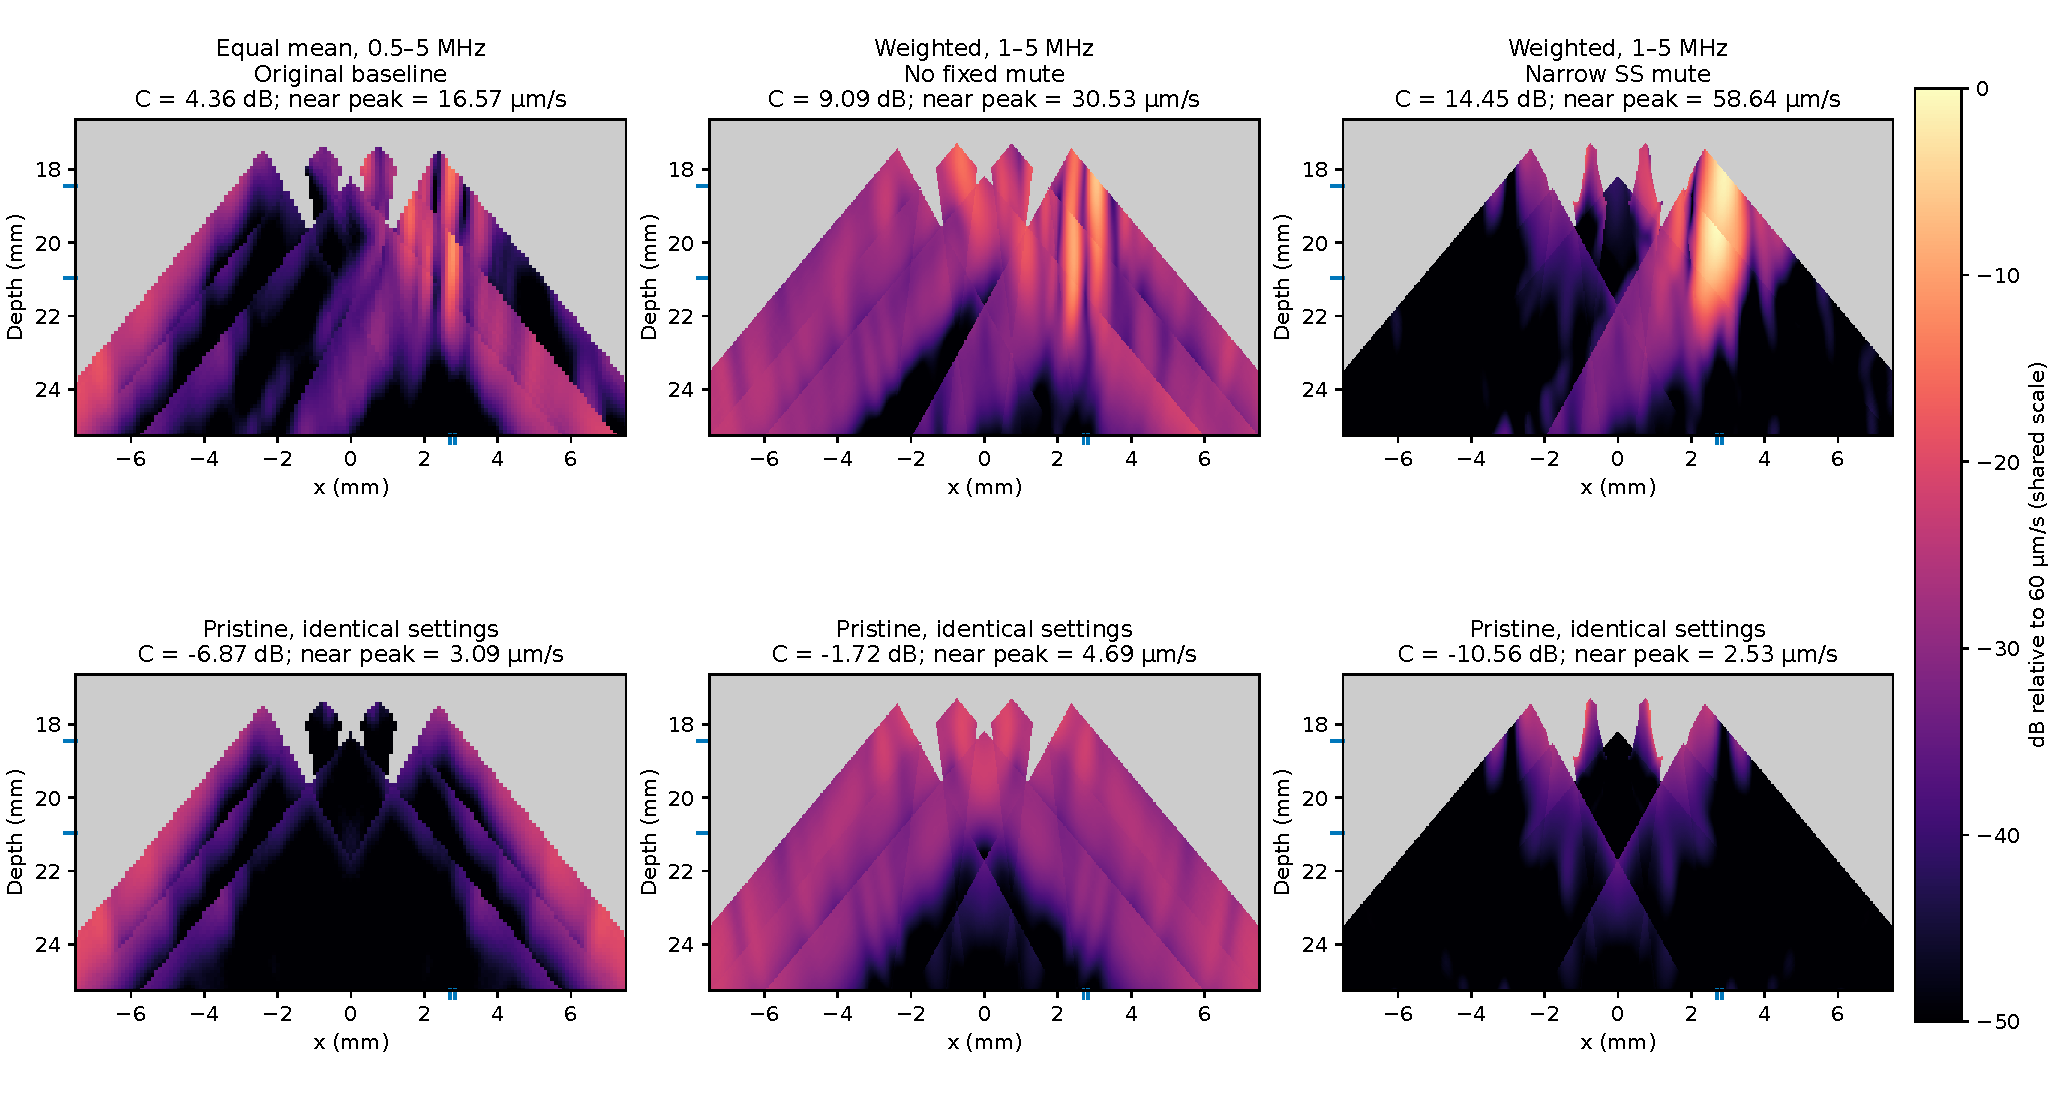
\includegraphics[width=\linewidth]{figures/review/partial_reassessment.pdf}
\caption{Partial-weld $S\mid SS$ improvement with pristine controls on a shared amplitude scale. Left: original equal-average image at 0.1 mm spacing. Centre: response weighting, 1--5 MHz and a 15\% angular threshold at 0.025 mm. Right: the same settings with the narrow $SS$ mute. Grey regions are unsupported.}
\label{combinedex:partial_reassessment}
\end{figure}

The mute raises contrast to 14.45 dB while retaining 96.9\% near support. The maximum is 58.64 $\mu$m/s at $(2.700,19.625)$ mm, 0.071 mm from the flaw. The pristine near-region maximum is 2.53 $\mu$m/s and its global maximum lies elsewhere. Muting changes phase cancellation and coherence, therefore the stronger image peak is an analysis improvement and not an increase in physical scattered energy. The mute was selected using this known flaw and does not establish that the entire reflected packet has been removed.

\subsection{Other paths}
The full analysis examined 324 paths across fixed source and receiver groups. Right-side reception does provide a useful  image: the right weld-surface source S3, at $(1.5,16.4)$ mm, with the 157 right receivers supports $S\mid LL$. This path uses direct shear illumination and a backwall-reflected longitudinal return. With response weighting, 1--5 MHz and a 15\% angular threshold, it gives 3.02 dB at 0.05 mm spacing. A narrow predicted-$LL$ mute raises this to 5.93 dB with 96.8\% near support. 

Other useful views include S3 with left receivers and unmuted $S\mid SS$, giving 11.49 dB locally and 11.03 dB in the wider field with about 96--97\% near support. S1 with left and weld-surface receivers gives $SLS\mid S$ contrasts of 15.80 and 4.01 dB, with 98.6\% and 100\% support. These local and wider checks use 0.05 and 0.25 mm grids respectively.

Not every promising local image survives these checks. S1 with right receivers and $SSL\mid SS$ reaches 9.24 dB locally using 1.5--5 MHz, but falls to $-25.24$ dB in the wider field, where the maximum is 21.14 mm from the flaw. Screening the full reflected packet also removes all near support for the complementary $S\mid LL$ view. These outcomes show why contrast, support, pristine controls and wider-field behaviour must be assessed together. The full results make the partial weld more promising, but it also shows that detection of the defect is dependent on all the different settings we use. More research into these settings and their justification must be done.

\section{Discussion}
\label{combinedex:discussion}
Both models provide LOF-only images from a calibrated laser-equivalent source and the resulting vertical surface velocity that an optical device such as an LDV could observe. No exact reference waveforms or response-weighted receiver mean is needed to obtain these main results. Considering these, both full and partial weld inspection are feasible for this modelled case and defects can be localized. What can't be shown is defect sizing, false negatives and spatial resolution of defect localization. It also does not prove these results translate to different geometries and defects.

Table~\ref{combinedex:synthesis} summarizes the acquisition choices. In the full weld, direct shear propagation and oblique shoulder illumination provide a strong lower-tip indication; side-surface reception can retain it. In the partial weld, the exposed weld surface provides useful generation and the backwall supplies a return route to outer receivers. Geometry, coupling and arrival timing explain this difference together. An aperture should therefore be selected for the intended mode and path, rather than specified only by its total number of sources or receivers. 

\par\medskip\noindent\begin{minipage}{\linewidth}\centering\small
\captionof{table}{Interpretation of the used acquisition strategies.}
\begin{tabularx}{\linewidth}{@{}l>{\raggedright\arraybackslash}X>{\raggedright\arraybackslash}X@{}}\toprule
Question & Full weld & Partial weld\\\midrule
Principal route & Direct $S\mid S$ & Direct illumination, backwall return $S\mid SS$\\
Useful reduced generation & Two shoulders & Three exposed weld-surface positions\\
Useful reception & Outer side surfaces & Left side for local view; both sides remain useful\\
Main coverage issue & Shoulder reduction retains 92.4\% near support & Two-source weld-only view retains 48.5\%; one source gives 95.8\%\\
Interpretation & Strong lower-tip localization & Local indication with explicit support/background trade-off\\
\bottomrule\end{tabularx}
\label{combinedex:synthesis}
\end{minipage}\par\medskip

\subsection{Source and receiver sensitivity}
Adding receivers can introduce stronger structural echoes as well as useful defect signals. These echoes may reduce contrast, even when the assumed wave paths are geometrically valid. Removing sources can improve the image but also leave more pixels unsupported. Image quality and coverage must therefore be assessed together.

A smaller measurement setup should still provide useful illumination and reception angles. The group comparisons identify useful source and receiver surfaces, but they do not find the minimum number of measurements needed. Further reductions should be tested over the same supported area, wider image fields, different flaws and realistic noise. 

\subsection{Filtering and image interpretation}
Filtering affects which signals reinforce during focusing. The common bandpass allows a consistent comparison between paths. A shorter low-pass improves the selected full-weld image, while the partial-weld improvement combines a different band with response weighting, a lower angular threshold and a narrow reflected-arrival mute. These settings work for the studied case, but have not been shown to be optimal for other flaws or measurements.

A shared colour scale makes image amplitudes comparable, but a bright region alone is not sufficient evidence of a flaw. The size of a bright feature depends on the wave field, measurement geometry, filtering and focusing, so it cannot be read directly as flaw size.

\subsection{Limitations}
The models assume homogeneous, isotropic steel and omit weld texture, residual stresses and temperature gradients, which is especially important considering the use case for Allseas. The two-dimensional approximation also excludes finite laser-line length, three-dimensional spreading and out-of-plane scattering. Optical access, surface reflectivity, signal dropout, positioning errors and detector noise are not included. Also the source calibration supports the mechanical approximation of laser generation, but does not validate that it corresponds to the real spectrum of a laser generation inside actual samples. Only one prescribed defect is studied, and its known position is used to calculate contrast and support. Detection probability and false-alarm rates therefore remain untested.

The next step is to test the proposed source positions, receiving surfaces and paths experimentally. The processing settings should then be kept fixed while testing different flaw positions, sizes and noise levels, with unsupported regions clearly shown.

\section{Conclusions}
The simulations show that the prescribed LOF can be localized in both weld states without subtracting a reference recording. Direct shear imaging works well in the full weld, while the partial weld benefits from weld-surface generation and a backwall-reflected return.

The selected full-weld image gives 12.79 dB contrast with complete near-flaw support. Using only shoulder sources and side receivers retains 9.61 dB with 92.4\% support. The revised partial-weld image gives 14.45 dB with 96.9\% support, compared with 9.09 dB for the same settings without the narrow reflected-arrival mute.

These results support the acoustic feasibility of laser-ultrasonic localization for the LOF defect. They also show that useful images require suitable wave paths, acquisition positions and processing settings. Experimental reliability and accurate flaw sizing still require further validation.

\FloatBarrier
\endgroup



